\documentclass[12pt]{article}

\pagestyle{empty}
\setlength{\topmargin}{0in}
\setlength{\headheight}{0in}
\setlength{\topsep}{0in}
\setlength{\textheight}{9in}
\setlength{\oddsidemargin}{0in}
\setlength{\evensidemargin}{0in}
\setlength{\textwidth}{6.5in}

\usepackage{palatino, graphicx,amssymb}

\newcommand{\ds}{\displaystyle}
\newcommand{\vs}[1]{\vspace{#1in}}
\renewcommand{\vss}[1]{\vspace*{#1in}}
\newcommand{\bvec}{{\mathbf b}}
\newcommand{\cvec}{{\mathbf c}}
\newcommand{\dvec}{{\mathbf d}}
\newcommand{\evec}{{\mathbf e}}
\newcommand{\fvec}{{\mathbf f}}
\newcommand{\qvec}{{\mathbf q}}
\newcommand{\uvec}{{\mathbf u}}
\newcommand{\vvec}{{\mathbf v}}
\newcommand{\wvec}{{\mathbf w}}
\newcommand{\xvec}{{\mathbf x}}
\newcommand{\yvec}{{\mathbf y}}
\newcommand{\zvec}{{\mathbf y}}
\newcommand{\zerovec}{{\mathbf 0}}
\newcommand{\real}{{\mathbb R}}
\newcommand{\twovec}[2]{\left[\begin{array}{r}#1 \\ #2
    \end{array}\right]}
\newcommand{\ctwovec}[2]{\left[\begin{array}{c}#1 \\ #2
   \end{array}\right]}
\newcommand{\threevec}[3]{\left[\begin{array}{r}#1 \\ #2 \\ #3
  \end{array}\right]}
\newcommand{\cthreevec}[3]{\left[\begin{array}{c}#1 \\ #2 \\ #3
    \end{array}\right]}
\newcommand{\fourvec}[4]{\left[\begin{array}{r}#1 \\ #2 \\ #3 \\ #4
    \end{array}\right]}
\newcommand{\cfourvec}[4]{\left[\begin{array}{c}#1 \\ #2 \\ #3 \\ #4
    \end{array}\right]}
\newcommand{\mattwo}[4]{\left[\begin{array}{rr}#1 & #2 \\ #3 & #4 \\ \end{array}\right]}
\renewcommand{\span}[1]{\text{Span}\{#1\}}
\newcommand{\bcal}{{\cal B}}
\newcommand{\ccal}{{\cal C}}
\newcommand{\scal}{{\cal S}}
\newcommand{\wcal}{{\cal W}}
\newcommand{\ecal}{{\cal E}}
\newcommand{\coords}[2]{\left\{#1\right\}_{#2}}
\newcommand{\gray}[1]{\color{gray}{#1}}
\newcommand{\lgray}[1]{\color{lightgray}{#1}}
\newcommand{\rank}{\text{rank}}
\newcommand{\col}{\text{Col}}
\newcommand{\nul}{\text{Nul}}

\begin{document}

\noindent
{\bf Mathematics 227} \\ 
{\bf Lab 3, Due: October 31, 2018}

\bigskip

\noindent
{\bf Instructions:} The exercises here should be completed in groups
of 2 or 3 students with one write-up submitted from each group.

\medskip
The JPEG compression algorithm begins by breaking an image into
$8\times8$ blocks of pixels.  Each pixel is represented as a color
using three coordinates in the luminance-chrominance color model
($YC_bC_r$).  For instance, here are the luminance values in one
$8\times8$ block.

\begin{center}
  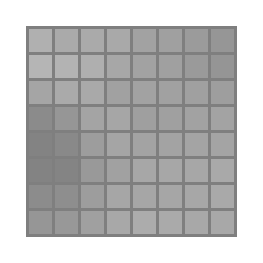
\includegraphics[scale=1.3]{jpeg-block-luminance.eps}
  \hspace*{24pt}
  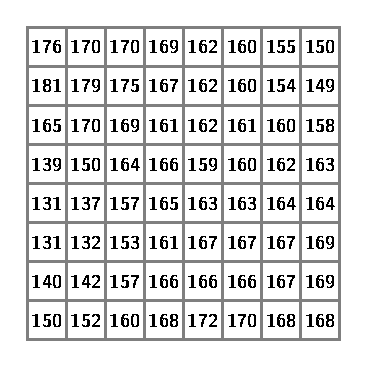
\includegraphics[scale=0.9]{jpeg-block-luminance-values.eps}
\end{center}

There are 64 values here, each represented by 8 bytes of computer
memory.  The compression algorithm works by finding a way of
representing this information using only a fraction of the 64 values. 

\bigskip
\begin{enumerate}
\item Let's look at the entries in the first column, which can be
  represented as a vector in $\real^8$:
  $$
  \xvec =
  \left[
    \begin{array}{c}
      x_0 \\ x_1 \\ x_2 \\ x_3 \\ x_4 \\ x_5 \\ x_6 \\ x_7 \\
    \end{array}
  \right] = 
  \left[
    \begin{array}{c}
      176 \\ 181 \\ 165 \\ 139 \\ 131 \\ 131 \\ 140 \\ 150 \\
    \end{array}
  \right].
  $$
  We can represent this graphically as:
  \begin{center}
    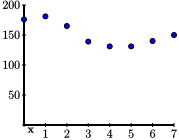
\includegraphics{jpeg-luminance-col-graph.eps}
  \end{center}

  Two things are important:
  \begin{itemize}
  \item There are not wide variations in these numbers across the
    column.
  \item If some of the values were to change slightly, our eyes would
    probably not notice because the pixels, when represented on a
    screen, are so small.
  \end{itemize}

  This suggests that we might be able to store the information more
  compactly using a different basis.

  The {\em Fourier transform} uses a new basis $\ccal$ for $\real^8$
  using the vectors
  $$
  \vvec_0 = \left[\begin{array}{c}
      \cos\left(\frac{(2\cdot 0+1)0\pi}{16}\right) \\
      \cos\left(\frac{(2\cdot 1+1)0\pi}{16}\right) \\
      \cos\left(\frac{(2\cdot 2+1)0\pi}{16}\right) \\
      \vdots \\
      \cos\left(\frac{(2\cdot 7+1)0\pi}{16}\right) 
      \end{array}\right], 
  \vvec_1 = \left[\begin{array}{c}
      \cos\left(\frac{(2\cdot 0+1)1\pi}{16}\right) \\
      \cos\left(\frac{(2\cdot 1+1)1\pi}{16}\right) \\
      \cos\left(\frac{(2\cdot 2+1)1\pi}{16}\right) \\
      \vdots \\
      \cos\left(\frac{(2\cdot 7+1)1\pi}{16}\right) 
      \end{array}\right], \ldots,
  \vvec_7 = \left[\begin{array}{c}
      \cos\left(\frac{(2\cdot 0+1)7\pi}{16}\right) \\
      \cos\left(\frac{(2\cdot 1+1)7\pi}{16}\right) \\
      \cos\left(\frac{(2\cdot 2+1)7\pi}{16}\right) \\
      \vdots\\
      \cos\left(\frac{(2\cdot 7+1)7\pi}{16}\right) 
      \end{array}\right]
    $$

    OK, this looks a little scary, but we can understand the vectors
    by looking at them graphically:

    \begin{center}
      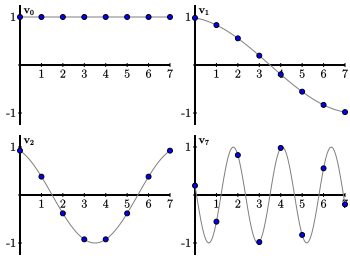
\includegraphics{jpeg-fourier-basis.eps}
    \end{center}

    Notice that $\vvec_0$ is constant, $\vvec_1$ varies slowly,
    $\vvec_2$ varies a little faster, and $\vvec_7$ varies quite
    rapidly.

    Representing a vector in these coordinates, we obtain
    $$
    \coords{\xvec}{\ccal} =
    \fvec = 
    \left[
      \begin{array}{c}
        F_0 \\ F_1 \\ F_2 \\ F_3 \\ F_4 \\ F_5 \\ F_6 \\ F_7 \\
      \end{array}
    \right],
    $$
    where components of $\fvec$ are called the {\em Fourier
      coefficients} of the 
    vector $\xvec$.  It turns out that $F_0$ is the average of the
    components of $\xvec$.

    Visit the page {\tt http://gvsu.edu/s/0Jd} where you can see the
    effect of changing three Fourier coefficients.

    What is the effect of changing $F_0$?

    \vs{1}
    How is the effect of changing $F_3$ different from the effect of
    changing $F_7$?

    \vs{1}
    If the vector $\xvec$ shows only small variations, what would you
    expect to be true of the Fourier coefficients $F_j$?

    \vs{1}

  \item Now go to the page {\tt gvsu.edu/s/0RF}, which is a page of
    Sage cells.  Evaluating the first cell will load some data and
    useful commands that are relevant to this lab.  After you evaluate
    the first cell, don't reuse it again.

    \newpage
    The first cell defines a matrix {\tt C} composed of
    the basis vectors $\vvec_0, \vvec_1,\ldots,\vvec_7$ and its
    inverse {\tt Cinv}.  The vector {\tt x}
    given above is also defined.  Find the vector $\fvec$ of Fourier
    coefficients of $\xvec$.

    \vs{1}
    What do you notice about the relative size of the Fourier
    coefficients?

    \vs{1}
    Form an approximation $\fvec_{\rm approx}$ to $\fvec$ by rounding
    the Fourier coefficients to the nearest integer and then setting
    $F_6$ and $F_7$ to 0.

    \vs{1}
    Now find the vector $\xvec_{\rm approx}$
    such that $\coords{\xvec_{\rm approx}}{\ccal} = \fvec_{\rm
      approx}$.

    \vs{1}
    Compare this vector to the original vector $\xvec$.  What is the
    largest difference in the components of $\xvec_{\rm approx}$ and
    $\xvec$?

    \vs{1}
    This is the central idea behind the compression algorithm:  we
    have thrown away two of the eight Fourier coefficients so that we
    save only 75\% of the Fourier data.  When we reconstruct $\xvec$,
    we have a very good approximation using only 75\% of the data.

    \newpage

  \item Let's return to our $8\times8$ block of luminance values.
    Each column of luminance values forms a vector in $\real^8$.
    Convert each column into its corresponding vector of Fourier
    coefficients and record the top row, consisting of the $F_0$
    components, below.

    \vs{1}
    Notice that the Fourier coefficients also don't change very much
    as you move across a row.  The next step in the compression
    algorithm is to view each row as a vector in $\real^8$ and
    represent that vector in terms of its Fourier coefficients.  This
    means that you are computing the Fourier coefficients of the
    Fourier coefficients.

    You can use the function {\tt double\_Fourier\_transform(luminance)}
    to do this.  Note the values in the upper-left $2\times2$ block
    below.

    \vs{1}

    Next, we will throw away some of the data contained in the Fourier
    coefficients.  Set any entry in this matrix less than 2 to 0 and
    round the rest of them to the nearest integer.  You can perform this
    operation using the function

    \noindent
    {\tt round\_matrix(double\_Fourier\_transform(luminance), 2)}.  Record 
    the upper $2\times2$ block below 
    and count how many nonzero entries there are in this matrix.

    \vs{1.5}
    You started with 64 pieces of data and now you are left with a
    much smaller number.  What fraction of the data have you thrown away?
    This is the compression ratio.

    \vs{1}
    \newpage
    If you call the rounded matrix {\tt ft\_approx}, you can recover
    the approximation to the luminance values with
    {\tt inverse\_double\_Fourier\_transform(ft\_approx)}.
    Write the
    four approximate luminance values from the upper-left $2\times2$
    corner and compare them to the original luminance values.  By how
    much do they differ?

    \vs{1}

    Compare the original luminance values to the approximated
    luminance values.  What is the largest difference that you find
    (Sage can help you do this)?

    \vs{1}

    Once again, this is the idea behind the compression algorithm.  We
    are saving only a small fraction of the original data yet we can
    reconstruct the colors with a fairly small error, which is
    probably less than our eyes would notice anyway.

    Above, we set the Fourier coefficients to 0 if they were below
    2.  If you choose a higher number, more of the Fourier
    coefficients will be set to 0.  This means you will be saving a
    smaller amount of data (the compression ratio goes up),
    but the errors in the reconstruction will be higher.
\end{enumerate}






\end{document}